\documentclass[conference]{IEEEtran}
\IEEEoverridecommandlockouts
% The preceding line is only needed to identify funding in the first footnote. If that is unneeded, please comment it out.
\usepackage{cite}
\usepackage{amsmath,amssymb,amsfonts}
\usepackage{algorithmic}
\usepackage{graphicx}
\usepackage{textcomp}
\usepackage{xcolor}
\usepackage[brazilian]{babel}
\usepackage[utf8]{inputenc}
\usepackage[T1]{fontenc}
\usepackage{listings}
\usepackage{color}
\usepackage{float}
\usepackage{multirow}
\usepackage{hyperref}

\definecolor{dkgreen}{rgb}{0,0.6,0}
\definecolor{gray}{rgb}{0.5,0.5,0.5}
\definecolor{mauve}{rgb}{0.58,0,0.82}

\lstset{frame=tb,
  language=Java,
  aboveskip=3mm,
  belowskip=3mm,
  showstringspaces=false,
  columns=flexible,
  basicstyle={\small\ttfamily},
  numbers=none,
  numberstyle=\tiny\color{gray},
  keywordstyle=\color{blue},
  commentstyle=\color{dkgreen},
  stringstyle=\color{mauve},
  breaklines=true,
  breakatwhitespace=true,
  tabsize=3
}
\lstset{language=Python}
\def\BibTeX{{\rm B\kern-.05em{\sc i\kern-.025em b}\kern-.08em
    T\kern-.1667em\lower.7ex\hbox{E}\kern-.125emX}}
\begin{document}

\title{Relatório do Laboratório 11: \\ Programação Dinâmica\\
}

\author{\IEEEauthorblockN{Isabelle Ferreira de Oliveira}
\IEEEauthorblockA{\textit{CT-213 - Engenharia da Computação 2020} \\
\textit{Instituto Tecnológico de Aeronáutica (ITA)}\\
São José dos Campos, Brasil \\
isabelle.ferreira3000@gmail.com}
}

\maketitle

\begin{abstract}
Esse relatório documenta a implementação de algoritmos de programação dinâmica no contexto de solução de um Processo Decisório de Markov (Markov Decision Process - MDP). Os algoritmos implementados serão avaliação de política (policy evaluation), iteração de política (policy iteration) e iteração de valor (value iteration), com o objetivo de avaliar políticas e determinar políticas ótimas para um grid world.
\end{abstract}

\begin{IEEEkeywords}
\textit{MDP}, policy evaluation, policy iteration, value iteration
\end{IEEEkeywords}

\section{Implementação}

\subsection{Implementação de Avaliação de Política}
Essa parte tratava-se da implementação da função \textit{policy\underline{\space}evaluation()}, presente no arquivo \textit{dynamic\underline{\space}programming.py}, fornecido pelo código base do professor. 

De maneira simples, essa função consiste na equação: $v_{k+1}\left ( s \right ) = \sum_{a\in A} \pi \left ( a|s \right ) r \left ( s, a \right ) + \gamma \sum_{a\in A} \sum_{s'\in S} \pi \left ( a|s \right ) p \left ( s' | s, a \right ) v_k \left ( s' \right )$, apresentada de forma bem semelhante no roteiro do laboratório \cite{roteiro}.

Para implementá-la, os estados $s$ (como também $s'$) se tornaram tuplas $(i, j)$, que foram iteradas por todo o grid world. Foram feitos loops também para iterar pelas ações $a$, e os resultados da equação acima foram somados ao valor associado ao estado em que se estava nessa iteração. 

\begin{enumerate}
\item $\pi \left ( a|s \right )$ era encontrado em \textit{policy};

\item $r \left ( s, a \right )$ estava em \textit{grid\underline{\space}world.reward()};

\item $p \left ( s' | s, a \right )$ estava em \textit{grid\underline{\space}world.transition\underline{\space}probability()};

\item $v_k \left ( s' \right )$ era a \textit{policy} para um outro estado $s'$.
\end{enumerate}

Vale ressaltar que, após um número definido previamente de iterações, ou após a convergência dos valores de $v_{k+1}(s)$, o loop era interrompido.

\subsection{Implementação de Iteração de Valor}
Essa parte tratava-se da implementação da função \textit{value\underline{\space}iteration()}, também presente no arquivo \textit{dynamic\underline{\space}programming.py}, fornecido pelo código base do professor.

Análogo a função anterior, essa função consiste na equação: $v_{k+1}\left ( s \right ) = max_{a \in A} \left (  r \left ( s, a \right ) + \gamma \sum_{s'\in S} p \left ( s' | s, a \right ) v_k \left ( s' \right ) \right )$, também presente no roteiro do laboratório \cite{roteiro}.

A implementação também se tornou bastante semelhante à função de Avaliação de Política, com os estados $s$ (como também $s'$) sendo tuplas $(i, j)$, que foram iteradas por todo o grid world, e loops para iterar pelas ações $a$, dessa vez buscando os valores máximos dos resultados da equação, para serem considerados como valor associado ao estado em que se estava nessa iteração. 

\begin{enumerate}
\item $r \left ( s, a \right )$ estava em \textit{grid\underline{\space}world.reward()};

\item $p \left ( s' | s, a \right )$ estava em \textit{grid\underline{\space}world.transition\underline{\space}probability()};

\item $v_k \left ( s' \right )$ era a \textit{policy} para um outro estado $s'$.
\end{enumerate}

Vale ressaltar que, após um número definido previamente de iterações, ou após a convergência dos valores de $v_{k+1}(s)$, o loop também era interrompido.

\subsection{Implementação de Iteração de Política}

\subsection{Comparação entre Grid Worlds diferentes}

\subsubsection{Função detect()}
Essa função tratava-se principalmente de três ações, a se saber: primeiro, era pré-processada a imagem de entrada (através da função \textit{preprocess\underline{\space}image()}; segundo, essa entrada pré-processada servia de entrada para rede, levando-a a um output; por fim, esse output era processado pelo algoritmo YOLO (através da função \textit{process\underline{\space}yolo\underline{\space}output()}), retornando, então, informações de onde estariam a bola e os dois postes da trave. A predição da rede do segundo passo foi implementado com a função \textit{predict()}, do Keras.

\subsubsection{Função preprocess\underline{\space}image()}
Essa função foi implementada com forte inspiração nas últimas três dicas da seção Dicas fornecidas pelo roteiro \cite{roteiro}, com o detalhe adicional de dividir os elementos do vetor da imagem por 255, a fim de transformar os valores RGB em valores de 0 a 1.

\subsubsection{Função process\underline{\space}yolo\underline{\space}output()}
Para processar o output através do algoritmo YOLO, percorreu-se a matriz output, guardando quais índices detinham a maior probabilidade de haver bola, a maior e a segunda maior probabilidade de haver postes de trave. Tendo posse desses índices, o restante das informações eram processados de acordo com as equações apresentadas na página 3 do roteiro do laboratório \cite{roteiro}. Por fim, era retornada essas informações processadas da bola e das duas traves.

\section{Resultados e Conclusões}

\subsection{Implementação da rede em Keras}
Ao se executar o script \textit{make\underline{\space}detector\underline{\space}network.py}, o resultado foi igual ao apresentado na Tabela 1 do roteiro \cite{roteiro}, comprovando a correta implementação da rede. Esse resultado pode ser visto nas Figuras \ref{tabela1} e \ref{tabela2}.

\begin{figure}[htbp]
\centering
\centerline{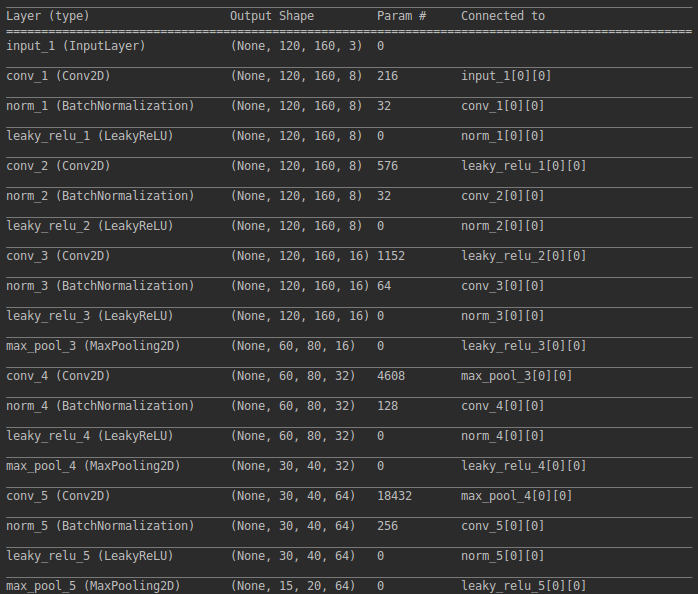
\includegraphics[scale=0.35]{imagens/tabela1.png}}
\caption{Primeira parte do summary da rede implementada em Keras.}.
\label{tabela1}
\end{figure}

\begin{figure}[htbp]
\centering
\centerline{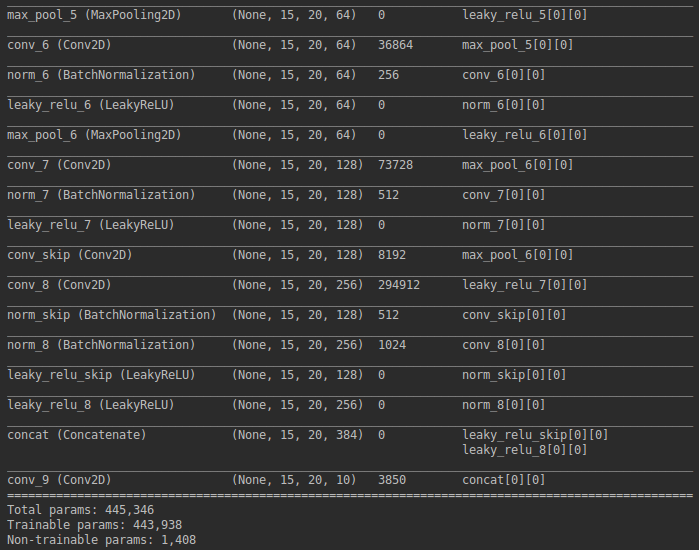
\includegraphics[scale=0.35]{imagens/tabela2.png}}
\caption{Segunda parte do summary da rede implementada em Keras, com a última linha da Figura \ref{tabela1} como primeira linha dessa figura.}.
\label{tabela2}
\end{figure} 

\subsection{Algoritmo YOLO}
Uma amostra das imagens geradas pelo algorito de detecção de objetos YOLO foram reproduzidos nas Figuras de \ref{imagem1_detection} a \ref{imagem7_detection}. Por essas imagens consegue-se observar o correto funcionamento do algoritmo, indicando que a implementação foi feita corretamente. Assim como esperado, então, conseguiu-se detectar a bola e os postes das traves nas imagens fornecidas pelo professor.

\begin{figure}[htbp]
\centering
\centerline{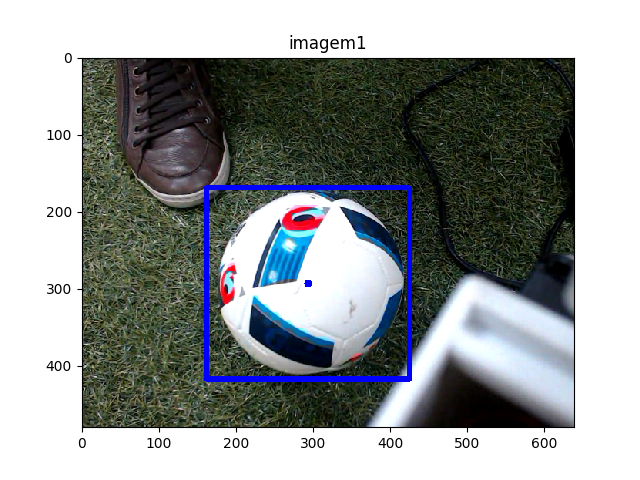
\includegraphics[scale=0.5]{imagens/imagem1_detection.png}}
\caption{Detecção de uma bola através do algoritmo de YOLO.}.
\label{imagem1_detection}
\end{figure}

\begin{figure}[htbp]
\centering
\centerline{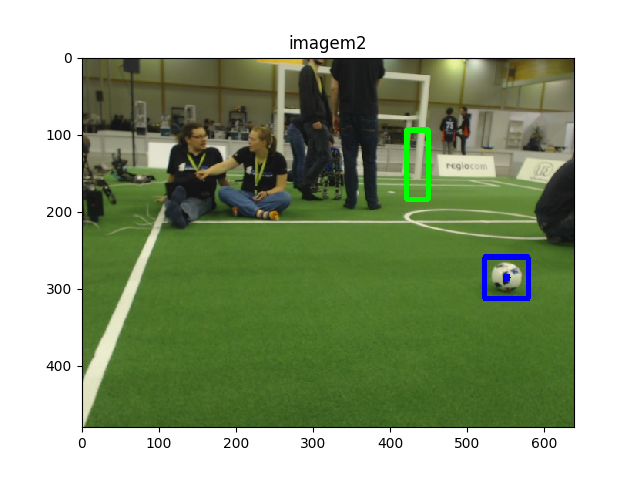
\includegraphics[scale=0.5]{imagens/imagem2_detection.png}}
\caption{Detecção de uma bola e de um dos postes da trave através do algoritmo de YOLO.}.
\label{imagem2_detection}
\end{figure}

\begin{figure}[htbp]
\centering
\centerline{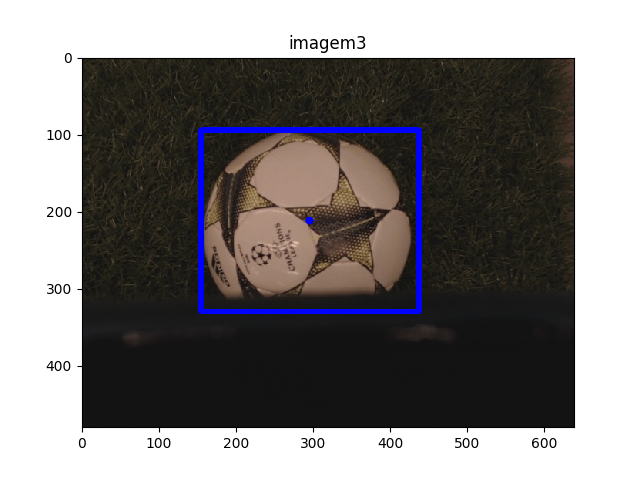
\includegraphics[scale=0.5]{imagens/imagem3_detection.png}}
\caption{Detecção de uma bola (mesmo que não completamente na imagem) através do algoritmo de YOLO.}.
\label{imagem3_detection}
\end{figure}

%\begin{figure}[htbp]
%\centering
%\centerline{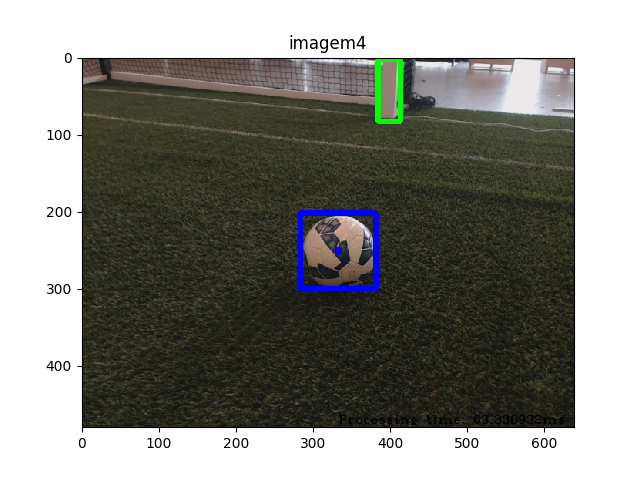
\includegraphics[scale=0.5]{imagens/imagem4_detection.png}}
%\caption{Custo do conjunto de validação, com o passar das épocas.}
%\label{imagem4_detection}
%\end{figure}

\begin{figure}[htbp]
\centering
\centerline{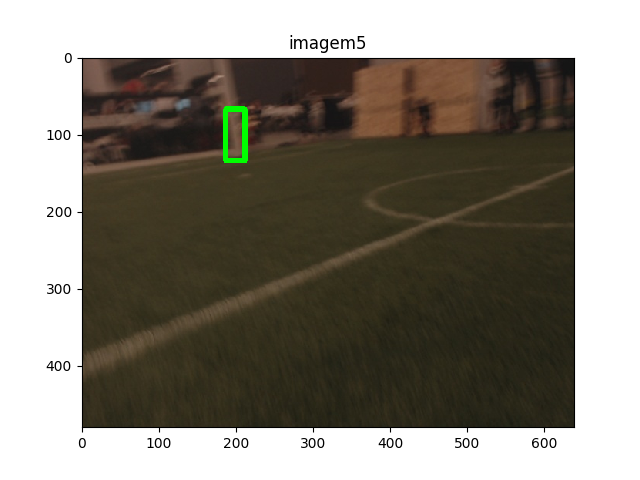
\includegraphics[scale=0.5]{imagens/imagem5_detection.png}}
\caption{Detecção de um poste de trave através do algoritmo de YOLO.}
\label{imagem5_detection}
\end{figure}

%\begin{figure}[htbp]
%\centering
%\centerline{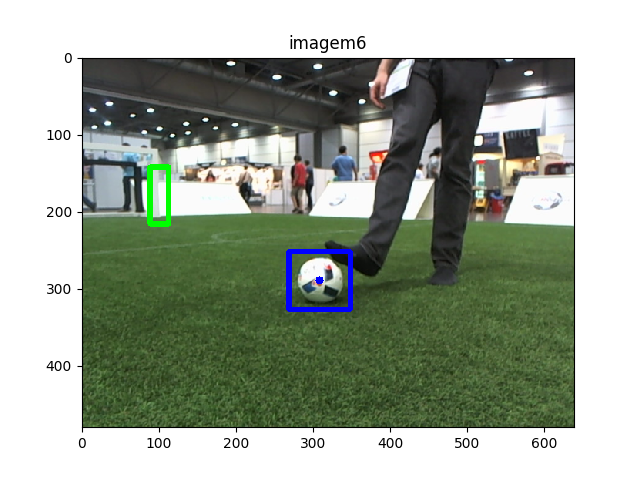
\includegraphics[scale=0.5]{imagens/imagem6_detection.png}}
%\caption{Número predito incorretamente.}
%\label{imagem6_detection}
%\end{figure}

\begin{figure}[htbp]
\centering
\centerline{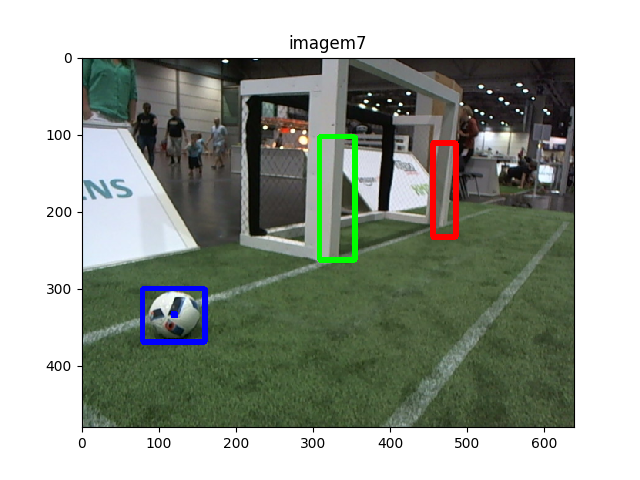
\includegraphics[scale=0.5]{imagens/imagem7_detection.png}}
\caption{Detecção de uma bola e dois postes da trave através do algoritmo de YOLO.}
\label{imagem7_detection}
\end{figure}

%\begin{figure}[htbp]
%\centering
%\centerline{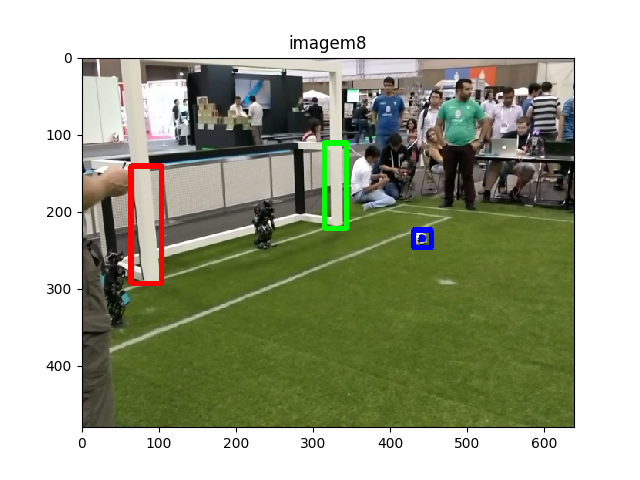
\includegraphics[scale=0.5]{imagens/imagem8_detection.png}}
%\caption{Número predito incorretamente.}
%\label{imagem8_detection}
%\end{figure}

%\begin{figure}[htbp]
%\centering
%\centerline{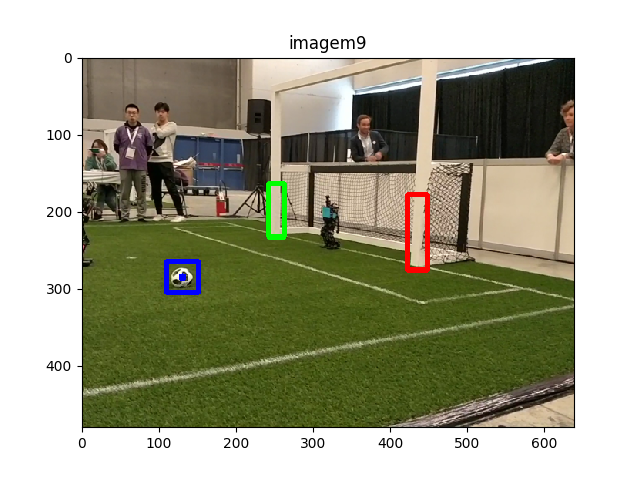
\includegraphics[scale=0.5]{imagens/imagem9_detection.png}}
%\caption{Número predito incorretamente.}
%\label{imagem9_detection}
%\end{figure}

%\begin{figure}[htbp]
%\centering
%\centerline{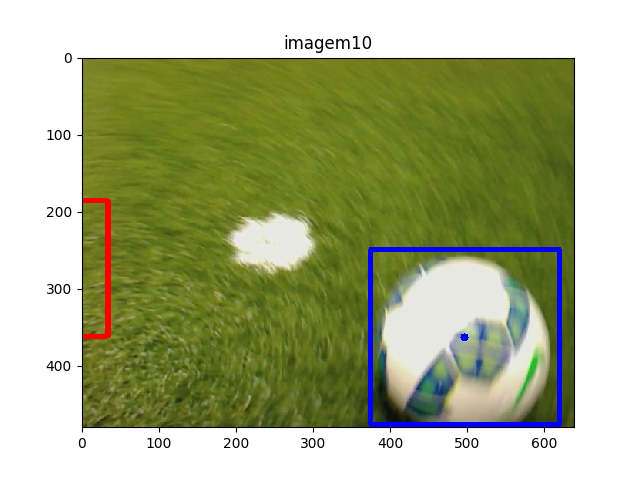
\includegraphics[scale=0.5]{imagens/imagem10_detection.png}}
%\caption{Número predito incorretamente.}
%\label{imagem10_detection}
%\end{figure}

Tendo em vista o que foi apresentado, pode-se notar, por fim, que a rede e o algoritmo YOLO realmente se demonstrou eficaz em realizar essa detecção de objetos em imagens.

\begin{thebibliography}{00}
\bibitem{roteiro} M. Maximo, ``Roteiro: Laboratório 11 - Programação Dinâmica''. Instituto Tecnológico de Aeronáutica, Departamento de Computação. CT-213, 2019.
\end{thebibliography}

\end{document}
